\documentclass[
11pt, % The default document font size, options: 10pt, 11pt, 12pt
%codirector, % Uncomment to add a codirector to the title page
]{charter} 


% El títulos de la memoria, se usa en la carátula y se puede usar el cualquier lugar del documento con el comando \ttitle
\titulo{Reconocimiento de eventos quirúrgicos a través de visión por computadora} 

% Nombre del posgrado, se usa en la carátula y se puede usar el cualquier lugar del documento con el comando \degreename
\posgrado{Maestría en Computación de Borde} 
%\posgrado{Carrera de Especialización en Internet de las Cosas} 
%\posgrado{Carrera de Especialización en Inteligencia Artificial}
%\posgrado{Maestría en Sistemas Embebidos} 
%\posgrado{Maestría en Internet de las cosas}

% Tu nombre, se puede usar el cualquier lugar del documento con el comando \authorname
% IMPORTANTE: no omitir titulaciones ni tildación en los nombres, también se recomienda escribir los nombres completos (tal cual los tienen en su documento)
\autor{Esp. Ing. Marín A. Brocca}

% El nombre del director y co-director, se puede usar el cualquier lugar del documento con el comando \supname y \cosupname y \pertesupname y \pertecosupname
\director{Dr. Ing. Axel Soto}
\pertenenciaDirector{UNS-CONICET} 
\codirector{Dr. Ing. Felix Sebastian Leo Thomsen} % para que aparezca en la portada se debe descomentar la opción codirector en los parámetros de documentclass
\pertenenciaCoDirector{UNS}

% Nombre del cliente, quien va a aprobar los resultados del proyecto, se puede usar con el comando \clientename y \empclientename
\cliente{Luciano Torun}
\empresaCliente{Wúru}
 
\fechaINICIO{24 de junio de 2025}		%Fecha de inicio de la cursada de GdP \fechaInicioName
\fechaFINALPlan{19 de agosto de 2025} 	%Fecha de final de cursada de GdP
\fechaFINALTrabajo{abril de 2026}	%Fecha de defensa pública del trabajo final


\begin{document}

\maketitle
\thispagestyle{empty}
\pagebreak


\thispagestyle{empty}
{\setlength{\parskip}{0pt}
\tableofcontents{}
}
\pagebreak



\section*{Registros de cambios}
\label{sec:registro}


\begin{table}[ht]
\label{tab:registro}
\centering
\begin{tabularx}{\linewidth}{@{}|c|X|c|@{}}
\hline
\rowcolor[HTML]{C0C0C0} 
Revisión & \multicolumn{1}{c|}{\cellcolor[HTML]{C0C0C0}Detalles de los cambios realizados} & Fecha      \\ \hline
0      & Creación del documento                                 &\fechaInicioName \\ \hline
1      & Se completa hasta el punto 9 inclusive                & 7 de julio de 2025\\ \hline
2      & Se completa hasta el punto 10 inclusive	& 15 de julio de 2025 \\ \hline
%		  Se puede agregar algo más \newline
%		  En distintas líneas \newline
%		  Así                                                    & {día} de {mes} de 202X \\ \hline
%3      & Se completa hasta el punto 12 inclusive                & {día} de {mes} de 202X \\ \hline
%4      & Se completa el plan	                                 & {día} de {mes} de 202X \\ \hline

% Si hay más correcciones pasada la versión 4 también se deben especificar acá

\end{tabularx}
\end{table}

\pagebreak



\section*{Acta de constitución del proyecto}
\label{sec:acta}

\begin{flushright}
Buenos Aires, \fechaInicioName
\end{flushright}

\vspace{2cm}

Por medio de la presente se acuerda con el \authorname\hspace{1px} que su Trabajo Final de la \degreename\hspace{1px} se titulará ``\ttitle'' y consistirá en la creación de un modelo de una aplicación basada en inteligencia artificial para la identificación de eventos en quirófanos por medio de visión por computadora. El trabajo tendrá un presupuesto preliminar estimado de 700 horas y un costo estimado de \$ 4000, con fecha de inicio el \fechaInicioName\hspace{1px} y fecha de presentación pública en el mes de  \fechaFinalName.

Se adjunta a esta acta la planificación inicial.

\vfill

% Esta parte se construye sola con la información que hayan cargado en el preámbulo del documento y no debe modificarla
\begin{table}[ht]
\centering
\begin{tabular}{ccc}
\begin{tabular}[c]{@{}c@{}}Dr. Ing. Ariel Lutenberg \\ Director posgrado FIUBA\end{tabular} & \hspace{2cm} & \begin{tabular}[c]{@{}c@{}}\clientename \\ \empclientename \end{tabular} \vspace{2.5cm} \\ 
\multicolumn{3}{c}{\begin{tabular}[c]{@{}c@{}} \supname \\ Director del Trabajo Final\end{tabular}} \vspace{2.5cm} \\
\end{tabular}
\end{table}

\section{1. Descripción técnica-conceptual del proyecto a realizar}
\label{sec:descripcion}

El presente proyecto se realiza en el marco del programa de vinculación con Wúru, empresa fundada en 2019 por un equipo con profunda experiencia en entornos hospitalarios que emergió con la visión de mejorar la eficiencia operativa en instituciones de salud. El foco de este equipo es la optimización continua de procesos mediante la capitalización del vasto volumen de datos generados por sistemas de registros médicos electrónicos (EMR) y equipos radiológicos. En función de esto, la empresa identificó desafíos críticos en el área quirúrgica: el alto costo asociado al tiempo ocioso de los quirófanos y la falta de precisión en el registro de eventos clave,  que impactan directamente en la planificación y utilización de recursos.

El problema central que se busca abordar radica en la naturaleza manual y propensa a errores de la documentación de eventos en las salas de operaciones. Actualmente, y dependiendo del sistema EMR empleado, tareas como el inicio y fin de una cirugía, la entrada o salida de pacientes o la limpieza de la sala dependen de la intervención manual del personal de enfermería. Esta dependencia no solo introduce inconsistencias y omisiones en los datos, sino que también genera una carga administrativa adicional y puede llevar a la duplicación de esfuerzos en diferentes sistemas. La consecuencia directa es el desaprovechamiento de los recursos del quirófano, un aumento en los costos operativos y una visibilidad limitada sobre el flujo real de trabajo. En la figura \ref{fig:lifecycle} se ejemplifica el ciclo de uso de un quirófano.

\begin{figure}[htpb]
	\centering 
	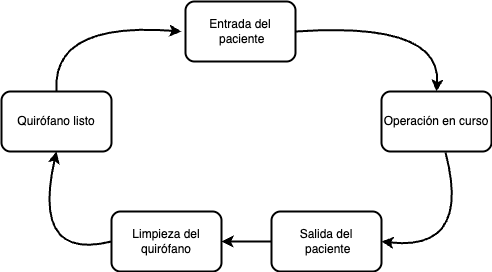
\includegraphics[width=.6\textwidth]{./Figuras/lifecycle.png}
	\caption{Ciclo de preparación y uso del quirófano.}
	\label{fig:lifecycle}
\end{figure}

En el mercado de soluciones hospitalarias existen diferentes alternativas que emplean en mayor o menor medida sistemas de grabaciones de video y voz con diferentes propósitos, como puede ser el monitoreo de eventos intraoperatorios, por ejemplo sangrado, conteo automático del instrumental empleado o capacitaciones a nuevo personal. Los principales inconvenientes de estas aplicaciones son su naturaleza cerrada, es decir, su limitada capacidad para ser integradas a sistemas locales, y el riesgo de dependencia del proveedor (\textit{vendor lock-in}).

Para resolver estos problemas se deben sortear los desafíos que incluyen la gestión del gran volumen de datos de video, la complejidad del etiquetado de eventos temporales (considerando variaciones de iluminación y perspectivas), el desarrollo de un modelo robusto capaz de generalizar a diversas condiciones de quirófano, y la construcción de una aplicación de demostración que refleje fielmente el potencial de la solución.

En la figura \ref{fig:Esquema} se presenta el diagrama en bloques del sistema propuesto. Se observa que la solución se fundamenta en la ingesta de videos provenientes de cámaras de vigilancia instaladas en las salas de operaciones. Estos videos son procesados por un modelo de visión por computadora entrenado para identificar eventos específicos como actividades de limpieza, el desarrollo de una operación y la entrada o salida de pacientes. A partir de esto, el sistema genera una salida estructurada que refleja el estado actual del quirófano. Dicha información se almacena en una base de datos operacional que alimenta una aplicación de demostración. Esta permite visualizar el estado del quirófano por medio de una interfaz intuitiva para la monitorización y la toma de decisiones operativas.

\begin{figure}[htpb]
	\centering 
	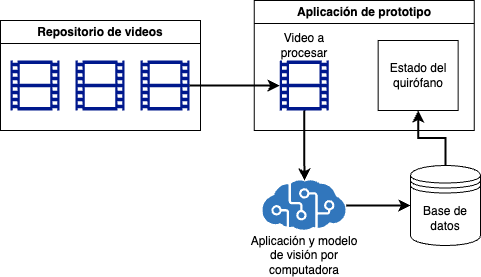
\includegraphics[width=.6\textwidth]{./Figuras/CEIA-GDP-Esquema.png}
	\caption{Diagrama en bloques del sistema a desarrollar.}
	\label{fig:Esquema}
\end{figure}

\section{2. Identificación y análisis de los interesados}
\label{sec:interesados}

\begin{table}[ht]
%\caption{Identificación de los interesados}
%\label{tab:interesados}
\begin{tabularx}{\linewidth}{@{}|l|X|X|l|@{}}
\hline
\rowcolor[HTML]{C0C0C0} 
Rol           & Nombre y Apellido & Organización 	& Puesto 	\\ \hline
Auspiciante       & \clientename      &\empclientename	&        CEO	\\ \hline
Cliente       & \clientename      &\empclientename	&        CEO	\\ \hline
Responsable   & \authorname       & FIUBA        	& Alumno 	\\ \hline
Colaborador       & Javier Roberts      &\empclientename	&        CTO	\\ \hline
Orientador    & \supname	      & \pertesupname 	& Director del Trabajo Final \\ \hline
Orientador    & \cosupname	      & \pertesupname 	& Codirector del Trabajo Final \\ \hline
Opositores    &    Aún no conocidos               &        -      	&        -	\\ \hline
Usuario final & Usuarios de la plataforma de gestión hospitalaria Wúru. & - & - \\ \hline

\end{tabularx}
\end{table}


\section{3. Propósito del proyecto}
\label{sec:proposito}

Desarrollar un prototipo de aplicación que, por medio de técnicas de visión por computadora, permita la automatización de los procesos asociados a la gestión de quirófanos.



\section{4. Alcance del proyecto}
\label{sec:alcance}

El proyecto incluye:
\begin{itemize}
	\item Relevamiento detallado de los requerimientos del cliente.
	\item Armado del dataset a partir de los datos crudos entregados por el cliente.
	\item Planteo de la tarea de visión por computadora a ser utilizada. 
	\item Selección, entrenamiento y ensayos con modelos de inteligencia artificial.
	\item Procesamiento del dataset.
	\item Desarrollo de un prototipo de aplicación de tres capas (backend, frontend y base de datos).
	\item Desarrollo de APIs para la integración entre la aplicación y el modelo.
	\item Ejecución de pruebas funcionales y de integración.
	\item Documentación y entrega de recomendaciones al cliente.
	\item Escritura de la memoria del trabajo final y defensa ante jurados.
	
\end{itemize}

Los siguientes elementos quedan fuera del alcance:
\begin{itemize}
	\item Implementación del sistema en producción.
	\item Integración del modelo con las aplicaciones del cliente.
	\item Integración de la aplicación con los sistemas de cámaras en los quirófanos. 

\end{itemize}



\section{5. Supuestos del proyecto}
\label{sec:supuestos}

Para el desarrollo del presente proyecto se supone que: 

\begin{itemize}
	\item Se dispondrá de la suficiente cantidad de videos para el correcto procesamiento e identificación de eventos..
	\item La calidad de los videos será la adecuada para su procesamiento.
	\item En caso de ser necesario, se contará con la ayuda de recursos por parte del cliente para el procesamiento y entrenamiento del modelo.
	\item Se dispondrá de materiales y/o de soporte académico para completar el proyecto.
	\item Se contará con el apoyo necesario del cliente cuando se requieran conocimientos específicos relacionados con la operatoria del quirófano.
\end{itemize}


\section{6. Requerimientos}
\label{sec:requerimientos}

\begin{enumerate}
	\item Requerimientos funcionales:
		\begin{enumerate}
			\item El modelo deberá reconocer 6 posibles estados del quirófano:
					\begin{enumerate}
						\item Quirófano vacío.
						\item Entrada de paciente.
						\item Operación en curso.
						\item Salida de paciente.
						\item Quirófano en limpieza.
						\item Otro.
					\end{enumerate}
			\item El estado identificado deberá ser guardado en una base de datos.
			\item El usuario debe poder procesar videos a demanda.
			\item La solución propuesta deberá indicar el grado de confianza de la detección del estado.
		\end{enumerate}
	\item Requerimientos asociados a los datos:
		\begin{enumerate}
			\item Se deberá resguardar la privacidad de los datos del hospital y de los pacientes.
			\item Por motivos de confidencialidad el almacenamiento de código se realizará en repositorios de acceso restringido.
		\end{enumerate}
	\item Requerimientos de documentación:
		\begin{enumerate}
		  \item Se desarrollará un informe de avance y una memoria final del proyecto.
		  \item Se entregarán recomendaciones para que el cliente pueda mejorar los procesos
		  de captura y recolección de datos.
		  \item El código se almacenará en la herramienta GitHub.
	    \end{enumerate}
	\item Requerimientos de la interfaz:
		\begin{enumerate}
		\item La interfaz de usuario será simple y clara y permitirá agregar un video para su procesamiento.
		\item El estado del quirófano será visible desde la interfaz de usario.
		\end{enumerate}	
\end{enumerate}

%Leyendo los requerimientos se debe poder interpretar cómo será el proyecto y su funcionalidad.

%Indicar claramente cuál es la prioridad entre los distintos requerimientos y si hay requerimientos opcionales. 


\section{7. Historias de usuarios (\textit{product backlog})}
\label{sec:backlog}

Las historias de usuarios se ponderan en base a las siguientes categorías:
\begin{itemize}
	\item Cantidad de trabajo a realizar para completar la tarea.
	\item Complejidad del trabajo requerido.
	\item Incertidumbre asociada a la actividad, es decir el riesgo de no poder completarla.
\end{itemize}

Para cada clase, los valores pueden ser 1 (bajo), 3 (medio) y 5 (alto). A las historias de usuario se les asigna un peso por cada categoría y luego estos valores se suman y se reemplazan por un número de la serie de Fibonacci (igual al resultado de la adición o inmediato superior).

En este proyecto se identifican los siguientes roles de usuarios:

\begin{itemize}
	\item Usuario administrativo: personal del hospital responsable de gestionar el uso del quirófano. 
	\item Administrador del sistema: responsable de la ejecución y monitoreo de los modelos y sistemas.
	\item Jefe de tecnología de Wúru: a cargo del correcto funcionamiento de la aplicación y su integración con los demás sistemas hospitalarios.
\end{itemize}

A continuación se detallan las historias de usuarios:

\begin{itemize}
	\item Como usuario administrativo, quiero poder identificar el estado del o de los quirófanos en cualquier momento para la correcta programación de cirugías . 
	\begin{itemize}
		\item Cantidad de trabajo a realizar: 5
		\item Complejidad del trabajo: 5
		\item Incertidumbre/riesgo: 3
		\item Ponderación final: 13 \textit{story points}
	\end{itemize}
\end{itemize}

\begin{itemize}
	\item Como administrador del sistema, quiero poder monitorear la efectividad del modelo como así también la \textit{performance} del sistema para evitar errores en la detección de eventos y la correcta asignación de estados al quirófano
	\begin{itemize}
		\item Cantidad de trabajo a realizar: 5
		\item Complejidad del trabajo: 5
		\item Incertidumbre/riesgo: 5
		\item Ponderación final: 21 \textit{story points}
	\end{itemize}
\end{itemize}

\begin{itemize}
	\item Como jefe de tecnología de Wúru, quiero saber qué técnicas y/o modelos
	de visión por computadora se ensayaron, para realizar a futuro la implementación en
	producción.
	\begin{itemize}
		\item Cantidad de trabajo a realizar: 3
		\item Complejidad del trabajo: 2
		\item Incertidumbre/riesgo: 1
		\item Ponderación final: 8 \textit{story points}
	\end{itemize}
\end{itemize}

%\begin{itemize}
%	\item Como administrador del sistema debo poder monitorear la efectividad del modelo como así también la \textit{performance} del sistema.
%	\begin{itemize}
%		\item Cantidad de trabajo a realizar: 5
%		\item Complejidad del trabajo: 5
%		\item Incertidumbre/riesgo: 5
%		\item Ponderación final: 21 \textit{story points}
%	\end{itemize}
%\end{itemize}

\section{8. Entregables principales del proyecto}
\label{sec:entregables}


Los entregables del proyecto son:

\begin{itemize}
	\item Informe para el cliente con resumen de ensayos, modelos y/o técnicas utilizadas, resultados	y recomendaciones para mejorar el proceso de captura de datos en el futuro.
	\item Código fuente.
	\item Plan del proyecto.
	\item Informe de avance.
	\item Memoria del trabajo final.

\end{itemize}


\section{9. Desglose del trabajo en tareas}
\label{sec:wbs}
\begin{enumerate}
	\item Configuración inicial y planificación. (80 h)
	\begin{enumerate}
		\item Definición del problema, requerimientos y categorías de eventos. (16 h)
		\item Creación del repositorio en GitHub, y de los entornos UV y MLflow.  (20 h)
		\item Configuración de control de versiones con DVC/Git LFS. (14 h)
		\item Selección y prueba inicial de una herramienta de etiquetado (CVAT/LabelStudio). (30 h)
	\end{enumerate}
	
	\item Preparación de datos y etiquetado. (190 h)
	\begin{enumerate}
		\item Análisis de videos, definición de eventos, preparación del dataset. (40 h)
		\item Definición del esquema de anotación (etiquetado). (30 h)
		\item Extracción de \textit{frames} y sincronización de \textit{timestamps}. (40 h)
		\item Etiquetado del quirófano 1. (40 h)
		\item Etiquetado del quirófano 2.  (40 h)

	\end{enumerate}
	
	\item Desarrollo del modelo. (128 h)
	\begin{enumerate}
		\item Realización de pruebas y selección del modelo base. (40 h)
		\item Configuración y prueba de la herramienta MLflow para seguimiento de experimentos. (8 h)
		\item Evaluación del modelo y ajuste de umbrales. (40 h)
		\item Evaluación final y métricas por estado. (40 h)
	\end{enumerate}
	
	\item Inferencia e integración (128 h)
	\begin{enumerate}
		\item Desarrollo de la aplicación prototipo. (40 h)
		\item Diseño del esquema de base de datos (SQLite/PostgreSQL). (8 h)
		\item Empaquetamiento del modelo y sus APIs en un contenedor Docker. (40 h)
		\item Realización de pruebas\textit{ end-to-end }(video → predicción → base de datos → dashboard). (40 h)
	\end{enumerate}
	
	\item Elaboración de documentos. (144 h)
	\begin{enumerate}
		\item Elaboración del informe de avance del proyecto. (5 h)
		\item Elaboración del video de demostración de la solución. (15 h)
		\item Confección de la memoria del trabajo final (TTF A). (20 h)
		\item Confección de la memoria del trabajo final (TTF B). (40 h)
		\item Aplicación de correcciones y ajustes en la memoria. (30 h)
		\item Documentación de código, herramientas y experimentos. (20 h)
		\item Creación del documento de recomendaciones para el cliente. (14 h)
	\end{enumerate}
	
	\item Presentación del trabajo. (30 horas)
	\begin{enumerate}
		\item Preparación de la presentación final y defensa pública del trabajo. (30 h)

	\end{enumerate}
	
\end{enumerate}

Cantidad total de horas: 700.


\section{10. Diagrama de Activity On Node}
\label{sec:AoN}
En la figura 3 se aprecia el diagrama de Activity on Node para este proyecto. Las tareas se
representan por medio de bloques interconectados con flechas para mostrar la dependencia que
hay entre ellas. El tiempo para cada actividad está expresado en horas y la duración del camino
crítico (identificado con color rojo) es de 501 h.

\begin{figure}[htpb]
\centering 
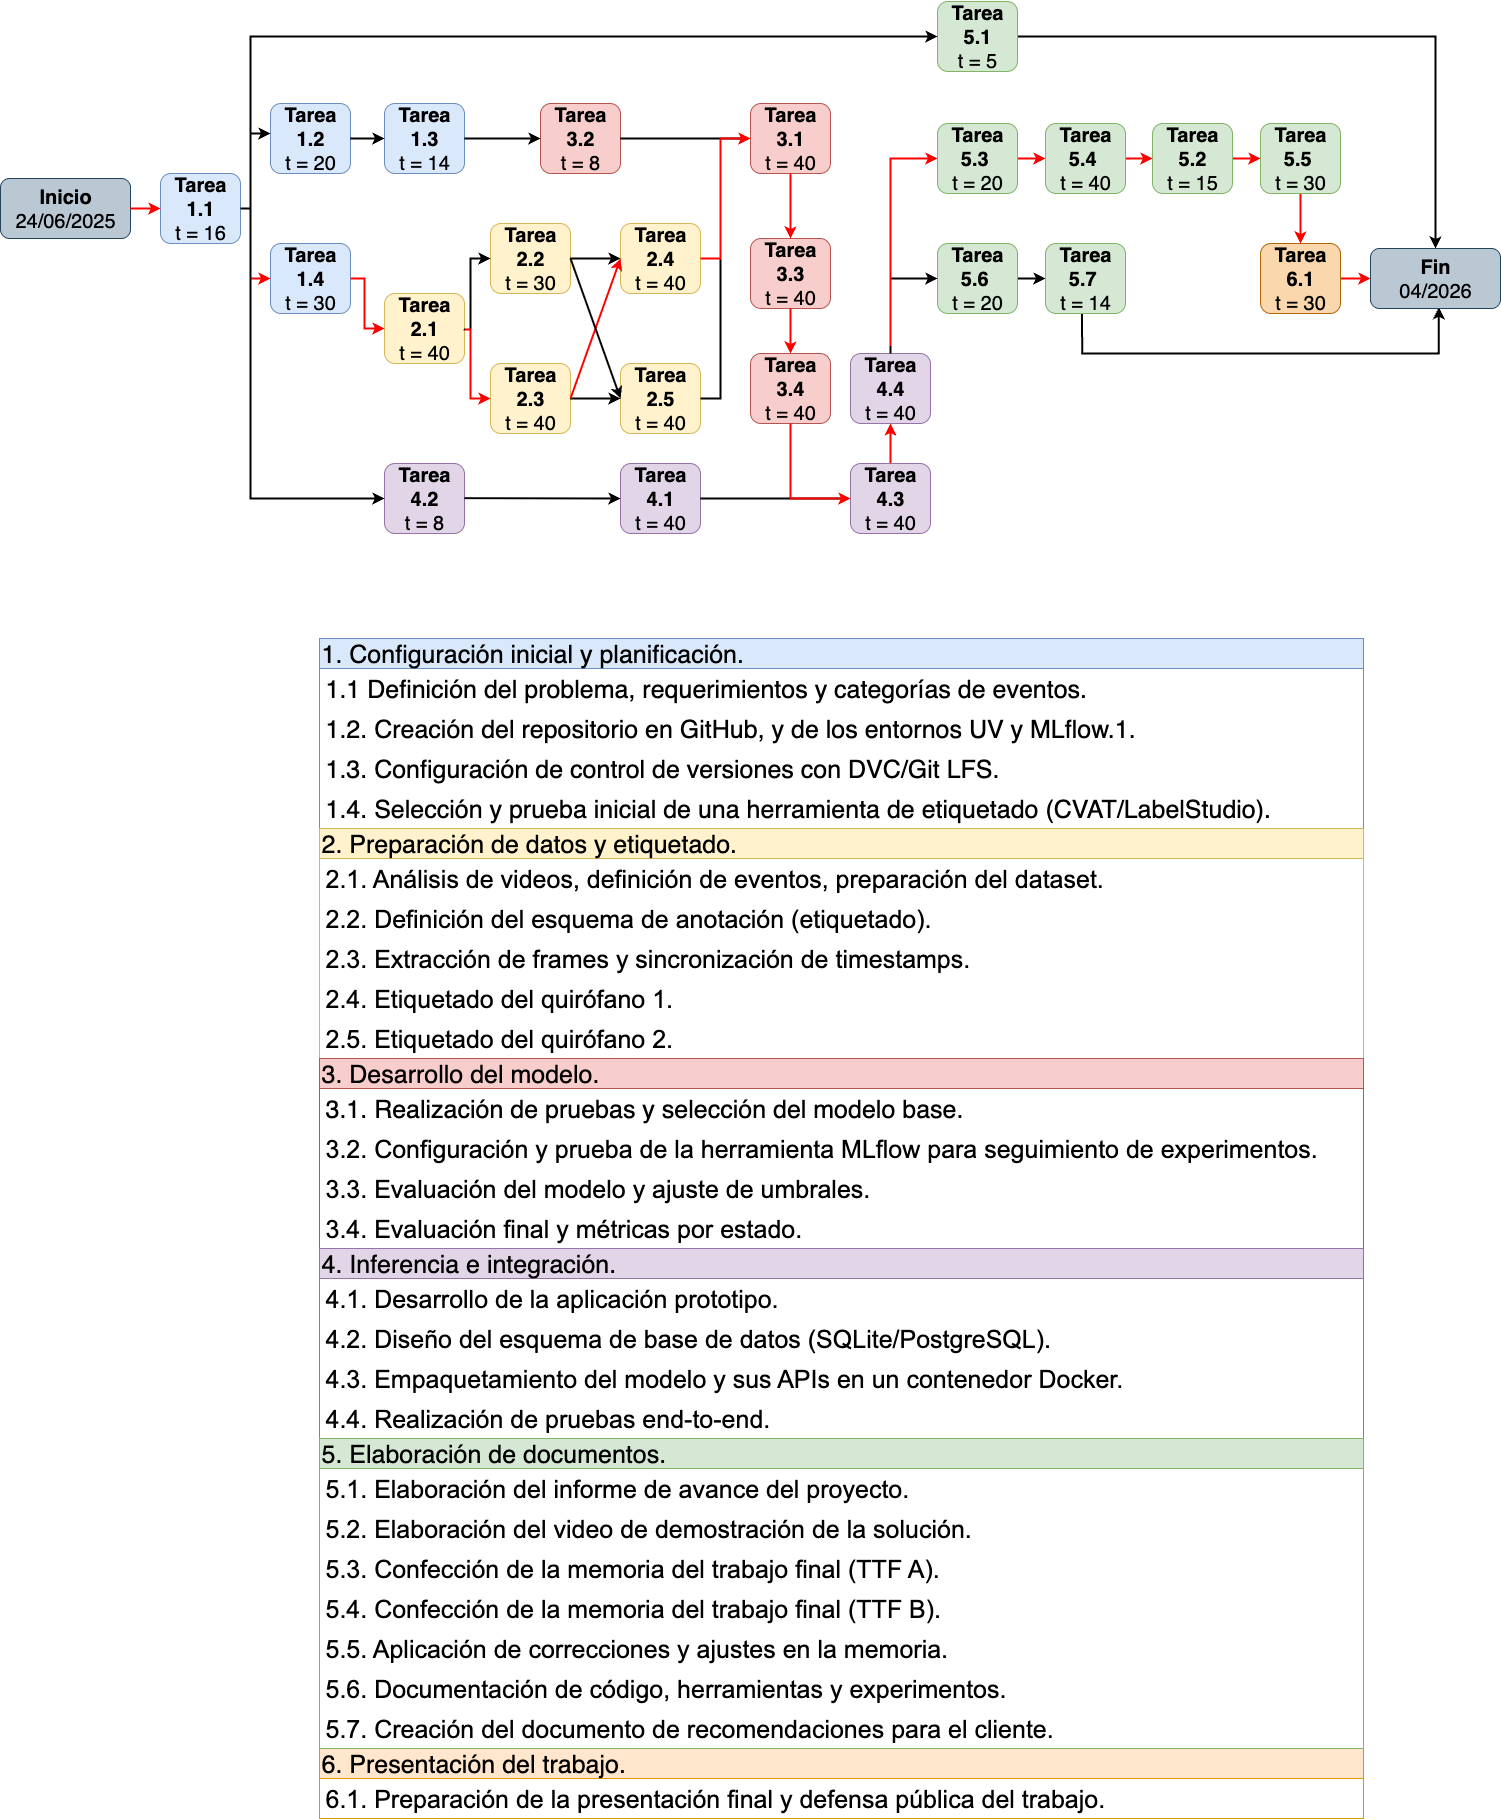
\includegraphics[width=1\textwidth]{./Figuras/CEIA-GDP-Esquema-AoN.table.png}
\caption{Diagrama de \textit{Activity on Node}.}
\label{fig:AoN}
\end{figure}



\section{11. Diagrama de Gantt}
\label{sec:gantt}
En base al las tareas identificadas y su orden de ejecución descripto en el diagrama \textit{Activity on Node}, se confeccionó el diagrama de Gantt del proyecto. Para una mejor lectura, en la tabla \ref{tab:wbs} se enumeran las actividades a ser realizadas, sus fechas de comienzo y finalización.  En la figura \ref{fig:gantt_chart} se observa el diagrama de Gantt propiamente dicho.
%\begin{table}[ht]
%	%\caption{Identificación de los interesados}
%	%\label{tab:interesados}
%	\begin{tabularx}{\linewidth}{@{}|l|X|X|l|@{}}
%		\hline
%		\rowcolor[HTML]{C0C0C0} 
%		Rol           & Nombre y Apellido & Organización 	& Puesto 	\\ \hline
%		Auspiciante       & \clientename      &\empclientename	&        CEO	\\ \hline
%		Cliente       & \clientename      &\empclientename	&        CEO	\\ \hline
%		Responsable   & \authorname       & FIUBA        	& Alumno 	\\ \hline
%		Colaborador       & Javier Roberts      &\empclientename	&        CTO	\\ \hline
%		Orientador    & \supname	      & \pertesupname 	& Director del Trabajo Final \\ \hline
%		Orientador    & \cosupname	      & \pertesupname 	& Codirector del Trabajo Final \\ \hline
%		Opositores    &    Aún no conocidos               &        -      	&        -	\\ \hline
%		Usuario final & Usuarios de la plataforma de gestión hospitalaria Wúru. & - & - \\ \hline
%		
%	\end{tabularx}
%\end{table}

\begin{table}[ht]
	\begin{tabularx}{\linewidth}{@{}|l|X|X|l|@{}}
		\hline
		\rowcolor[HTML]{C0C0C0}
		\textbf{Nombre de tarea} & \textbf{Inicio} & \textbf{Fin} \\ \hline
		\multicolumn{3}{|l|}{\textbf{1. Configuración inicial y planificación.}} \\ \hline
		1.1 Definición del problema. & 24/06/25 & 01/07/25 \\ \hline
		1.2 Creación del repositorio. & 02/07/25 & 10/07/25 \\ \hline
		1.3 Configuración de DVC/Git LFS. & 11/07/25 & 17/07/25 \\ \hline
		1.4 Selección y prueba de herramienta de etiquetado. & 02/07/25 & 15/07/25 \\ \hline
		\multicolumn{3}{|l|}{\textbf{2. Preparación de datos y etiquetado.}} \\ \hline
		2.1 Análisis de videos, definición de eventos. & 16/07/25 & 04/08/25 \\ \hline
		2.2 Definición del esquema de etiquetado. & 05/08/25 & 18/08/25 \\ \hline
		2.3 Extracción de \textit{frames}. & 05/08/25 & 22/08/25 \\ \hline
		2.4 Etiquetado del quirófano 1. & 25/08/25 & 11/09/25 \\ \hline
		2.5 Etiquetado del quirófano 2. & 25/08/25 & 11/09/25 \\ \hline
		\multicolumn{3}{|l|}{\textbf{3. Desarrollo del modelo.}} \\ \hline
		3.1 Realización de pruebas y selección del modelo base. & 12/09/25 & 01/10/25 \\ \hline
		3.2 Configuración de MLflow. & 18/07/25 & 22/07/25 \\ \hline
		3.3 Evaluación del modelo y ajuste de umbrales. & 02/10/25 & 21/10/25 \\ \hline
		3.4 Evaluación final y métricas por estado. & 22/10/25 & 10/11/25 \\ \hline
		\multicolumn{3}{|l|}{\textbf{4. Inferencia e integración.}} \\ \hline
		4.1 Desarrollo de la aplicación prototipo. & 07/09/25 & 24/09/25 \\ \hline
		4.2 Diseño del esquema de base de datos. & 02/09/25 & 04/09/25 \\ \hline
		4.3 Empaquetamiento del modelo y sus APIs. & 11/11/25 & 20/11/25 \\ \hline
		4.4 Realización de pruebas \textit{end-to-end}. & 25/11/25 & 01/12/25 \\ \hline
		\multicolumn{3}{|l|}{\textbf{5. Elaboración de documentos.}} \\ \hline
		5.1 Elaboración del informe de avance del proyecto. & 02/10/25 & 03/10/25 \\ \hline
		5.2 Elaboración del video de demostración de la solución. & 15/03/26 & 01/04/26 \\ \hline
		5.3 Confección de la memoria (TTF A). & 05/12/25 & 21/12/25 \\ \hline
		5.4 Confección de la memoria (TTF B). & 01/03/26 & 15/03/26 \\ \hline
		5.5 Aplicación de correcciones y ajustes en la memoria. & 01/04/26 & 10/04/26 \\ \hline
		5.6 Documentación de código, herramientas y experimentos. & 19/12/25 & 30/12/25 \\ \hline
		5.7 Creación del documento de recomendaciones. & 31/12/25 & 07/01/26 \\ \hline
		\multicolumn{3}{|l|}{\textbf{6. Presentación del trabajo.}} \\ \hline
		6.1 Presentación final y defensa pública del trabajo. & 12/04/26 & 20/04/26 \\ \hline
	\end{tabularx}
	\caption{Resumen de tareas del cronograma de trabajo.}
	\label{tab:wbs}
\end{table}


\clearpage % Flush pending floats before switching to landscape
\begin{landscape}
	\begin{figure}[ht!]
		\centering
		\begin{ganttchart}[
			hgrid,
			x unit=0.05cm,
			y unit title=0.5cm,
			y unit chart=0.42cm,
			time slot format=isodate,
			time slot unit=day,
			bar height=0.4,
			group height=0.4,
			milestone height=0.4,
			title height=0.7,
			bar/.style={fill=blue!20},
			group/.style={fill=blue!40},
			milestone/.style={fill=gray},
			bar label font=\small,
			group label font=\small\bfseries,
			milestone label font=\small
			]{2025-06-24}{2026-04-26}
			\gantttitlecalendar{year, month=shortname} \\
			% Milestones
			\ganttmilestone[name=start]{Inicio}{2025-06-24} \\
			
			
			% Add vertical rules for each month start
			\ganttvrule[vrule/.style={draw=gray!50, dashed}]{}{2025-07-01} % July
			\ganttvrule[vrule/.style={draw=gray!50, dashed}]{}{2025-08-01} % August
			\ganttvrule[vrule/.style={draw=gray!50, dashed}]{}{2025-09-01} % September
			\ganttvrule[vrule/.style={draw=gray!50, dashed}]{}{2025-10-01} % October
			\ganttvrule[vrule/.style={draw=gray!50, dashed}]{}{2025-11-01} % November
			\ganttvrule[vrule/.style={draw=gray!50, dashed}]{}{2025-12-01} % December
			\ganttvrule[vrule/.style={draw=gray!50, dashed}]{}{2026-01-01} % January
			\ganttvrule[vrule/.style={draw=gray!50, dashed}]{}{2026-02-01} % February
			\ganttvrule[vrule/.style={draw=gray!50, dashed}]{}{2026-03-01} % March
			\ganttvrule[vrule/.style={draw=gray!50, dashed}]{}{2026-04-01} % April
			
			
			% Phase 1
			\ganttgroup[name=group_1]{1. Configuración inicial y planificación}{2025-06-24}{2025-07-15} \\
			\ganttbar[name=task_1_1]{1.1 Definición del problema}{2025-06-24}{2025-07-01} \\
			\ganttbar[name=task_1_2]{1.2 Creación del repositorio}{2025-07-02}{2025-07-10} \\
			\ganttbar[name=task_1_3]{1.3 Configuración de DVC/Git LFS}{2025-07-11}{2025-07-17} \\
			\ganttbar[name=task_1_4]{1.4 Selección y prueba de herramienta de etiquetado}{2025-07-02}{2025-07-15} \\
			\ganttlink{task_1_1}{task_1_2}
			\ganttlink{task_1_1}{task_1_4}
			\ganttlink{task_1_2}{task_1_3}
			
			
			\ganttvrule[vrule/.style={draw=gray!50, dashed}]{}{2025-07-01} % July
\ganttvrule[vrule/.style={draw=gray!50, dashed}]{}{2025-08-01} % August
\ganttvrule[vrule/.style={draw=gray!50, dashed}]{}{2025-09-01} % September
\ganttvrule[vrule/.style={draw=gray!50, dashed}]{}{2025-10-01} % October
\ganttvrule[vrule/.style={draw=gray!50, dashed}]{}{2025-11-01} % November
\ganttvrule[vrule/.style={draw=gray!50, dashed}]{}{2025-12-01} % December
\ganttvrule[vrule/.style={draw=gray!50, dashed}]{}{2026-01-01} % January
\ganttvrule[vrule/.style={draw=gray!50, dashed}]{}{2026-02-01} % February
\ganttvrule[vrule/.style={draw=gray!50, dashed}]{}{2026-03-01} % March
\ganttvrule[vrule/.style={draw=gray!50, dashed}]{}{2026-04-01} % April
			
			% Phase 2
			\ganttgroup[name=group_2]{2. Preparación de datos y etiquetado}{2025-07-16}{2025-09-11} \\
			\ganttbar[name=task_2_1]{2.1 Análisis de videos, definición de eventos}{2025-07-16}{2025-08-04} \\
			\ganttbar[name=task_2_2]{2.2 Definición del esquema de etiquetado}{2025-08-05}{2025-08-18} \\
			\ganttbar[name=task_2_3]{2.3 Extracción de \textit{frames}}{2025-08-05}{2025-08-22} \\
			\ganttbar[name=task_2_4]{2.4 Etiquetado del quirófano 1}{2025-08-25}{2025-09-11} \\
			\ganttbar[name=task_2_5]{2.5 Etiquetado del quirófano 2}{2025-08-25}{2025-09-11} \\
			\ganttlink{task_1_4}{task_2_1}
			\ganttlink{task_2_1}{task_2_2}
			\ganttlink{task_2_1}{task_2_3}
			\ganttlink{task_2_2}{task_2_4}
			\ganttlink{task_2_3}{task_2_4}
			\ganttlink{task_2_3}{task_2_5}
			
						\ganttvrule[vrule/.style={draw=gray!50, dashed}]{}{2025-07-01} % July
			\ganttvrule[vrule/.style={draw=gray!50, dashed}]{}{2025-08-01} % August
			\ganttvrule[vrule/.style={draw=gray!50, dashed}]{}{2025-09-01} % September
			\ganttvrule[vrule/.style={draw=gray!50, dashed}]{}{2025-10-01} % October
			\ganttvrule[vrule/.style={draw=gray!50, dashed}]{}{2025-11-01} % November
			\ganttvrule[vrule/.style={draw=gray!50, dashed}]{}{2025-12-01} % December
			\ganttvrule[vrule/.style={draw=gray!50, dashed}]{}{2026-01-01} % January
			\ganttvrule[vrule/.style={draw=gray!50, dashed}]{}{2026-02-01} % February
			\ganttvrule[vrule/.style={draw=gray!50, dashed}]{}{2026-03-01} % March
			\ganttvrule[vrule/.style={draw=gray!50, dashed}]{}{2026-04-01} % April
			% Phase 3
			\ganttgroup[name=group_3]{3. Desarrollo del modelo}{2025-09-12}{2025-11-10} \\
			\ganttbar[name=task_3_1]{3.1 Realización de pruebas y selección del modelo base}{2025-09-12}{2025-10-01} \\
			\ganttbar[name=task_3_2]{3.2 Configuración de MLflow}{2025-07-18}{2025-07-22} \\
			\ganttbar[name=task_3_3]{3.3 Evaluación del modelo y ajuste de umbrales}{2025-10-02}{2025-10-21} \\
			\ganttbar[name=task_3_4]{3.4 Evaluación final y métricas por estado}{2025-10-22}{2025-11-10} \\
			\ganttlink{task_1_3}{task_3_2}
			\ganttlink{task_2_4}{task_3_1}
			\ganttlink{task_2_5}{task_3_1}
			\ganttlink{task_3_1}{task_3_3}
			\ganttlink{task_3_3}{task_3_4}
			\ganttlink{task_3_2}{task_3_1}
			
						\ganttvrule[vrule/.style={draw=gray!50, dashed}]{}{2025-07-01} % July
			\ganttvrule[vrule/.style={draw=gray!50, dashed}]{}{2025-08-01} % August
			\ganttvrule[vrule/.style={draw=gray!50, dashed}]{}{2025-09-01} % September
			\ganttvrule[vrule/.style={draw=gray!50, dashed}]{}{2025-10-01} % October
			\ganttvrule[vrule/.style={draw=gray!50, dashed}]{}{2025-11-01} % November
			\ganttvrule[vrule/.style={draw=gray!50, dashed}]{}{2025-12-01} % December
			\ganttvrule[vrule/.style={draw=gray!50, dashed}]{}{2026-01-01} % January
			\ganttvrule[vrule/.style={draw=gray!50, dashed}]{}{2026-02-01} % February
			\ganttvrule[vrule/.style={draw=gray!50, dashed}]{}{2026-03-01} % March
			\ganttvrule[vrule/.style={draw=gray!50, dashed}]{}{2026-04-01} % April
			% Phase 4
			\ganttgroup[name=group_4]{4. Inferencia e integración}{2025-07-02}{2025-12-18} \\
			\ganttbar[name=task_4_1]{4.1 Desarrollo de la aplicación prototipo}{2025-09-07}{2025-09-24} \\
			\ganttbar[name=task_4_2]{4.2 Diseño del esquema de base de datos}{2025-09-02}{2025-09-04} \\
			\ganttbar[name=task_4_3]{4.3 Empaquetamiento del modelo y sus APIs}{2025-11-11}{2025-11-20} \\
			\ganttbar[name=task_4_4]{4.4 Realización de pruebas \textit{end-to-end}}{2025-11-20}{2025-12-01} \\
			\ganttlink{task_1_1}{task_4_2}
			\ganttlink{task_4_2}{task_4_1}
			\ganttlink{task_3_4}{task_4_3}
			\ganttlink{task_4_3}{task_4_4}
			
						\ganttvrule[vrule/.style={draw=gray!50, dashed}]{}{2025-07-01} % July
			\ganttvrule[vrule/.style={draw=gray!50, dashed}]{}{2025-08-01} % August
			\ganttvrule[vrule/.style={draw=gray!50, dashed}]{}{2025-09-01} % September
			\ganttvrule[vrule/.style={draw=gray!50, dashed}]{}{2025-10-01} % October
			\ganttvrule[vrule/.style={draw=gray!50, dashed}]{}{2025-11-01} % November
			\ganttvrule[vrule/.style={draw=gray!50, dashed}]{}{2025-12-01} % December
			\ganttvrule[vrule/.style={draw=gray!50, dashed}]{}{2026-01-01} % January
			\ganttvrule[vrule/.style={draw=gray!50, dashed}]{}{2026-02-01} % February
			\ganttvrule[vrule/.style={draw=gray!50, dashed}]{}{2026-03-01} % March
			\ganttvrule[vrule/.style={draw=gray!50, dashed}]{}{2026-04-01} % April
			% Phase 5
			\ganttgroup[name=group_5]{5. Elaboración de documentos}{2025-07-02}{2026-02-11} \\
			\ganttbar[name=task_5_1]{5.1 Elaboración del informe de avance del proyecto}{2025-10-02}{2025-10-03} \\
			\ganttbar[name=task_5_2]{5.2 Elaboración del video de demostración de la solución}{2026-03-15}{2026-04-01} \\
			\ganttbar[name=task_5_3]{5.3 Confección de la memoria (TTF A)}{2025-12-04}{2025-12-21} \\
			\ganttbar[name=task_5_4]{5.4 Confección de la memoria (TTF B)}{2026-03-01}{2026-03-15} \\
			\ganttbar[name=task_5_5]{5.5 Aplicación de correcciones y ajustes en la memoria}{2026-04-01}{2026-04-10} \\
			\ganttbar[name=task_5_6]{5.6 Documentación de código, herramientas y experimentos}{2025-12-19}{2025-12-30} \\
			\ganttbar[name=task_5_7]{5.7 Creación del documento de recomendaciones}{2025-12-31}{2026-01-07} \\
			\ganttlink{task_1_1}{task_5_1}
			\ganttlink{task_4_4}{task_5_6}
			\ganttlink{task_4_4}{task_5_3}
			\ganttlink{task_5_3}{task_5_4}
			\ganttlink{task_5_4}{task_5_2}
			\ganttlink{task_5_2}{task_5_5}
			\ganttlink{task_5_6}{task_5_7}
			
						\ganttvrule[vrule/.style={draw=gray!50, dashed}]{}{2025-07-01} % July
			\ganttvrule[vrule/.style={draw=gray!50, dashed}]{}{2025-08-01} % August
			\ganttvrule[vrule/.style={draw=gray!50, dashed}]{}{2025-09-01} % September
			\ganttvrule[vrule/.style={draw=gray!50, dashed}]{}{2025-10-01} % October
			\ganttvrule[vrule/.style={draw=gray!50, dashed}]{}{2025-11-01} % November
			\ganttvrule[vrule/.style={draw=gray!50, dashed}]{}{2025-12-01} % December
			\ganttvrule[vrule/.style={draw=gray!50, dashed}]{}{2026-01-01} % January
			\ganttvrule[vrule/.style={draw=gray!50, dashed}]{}{2026-02-01} % February
			\ganttvrule[vrule/.style={draw=gray!50, dashed}]{}{2026-03-01} % March
			\ganttvrule[vrule/.style={draw=gray!50, dashed}]{}{2026-04-01} % April
			
			% Phase 6
			\ganttgroup[name=group_6]{6. Presentación del trabajo}{2026-04-12}{2026-04-20} \\
			\ganttbar[name=task_6_1]{6.1 Presentación final y defensa pública del trabajo}{2026-04-12}{2026-04-20} \\
			\ganttlink{task_5_5}{task_6_1}
			
						\ganttvrule[vrule/.style={draw=gray!50, dashed}]{}{2025-07-01} % July
			\ganttvrule[vrule/.style={draw=gray!50, dashed}]{}{2025-08-01} % August
			\ganttvrule[vrule/.style={draw=gray!50, dashed}]{}{2025-09-01} % September
			\ganttvrule[vrule/.style={draw=gray!50, dashed}]{}{2025-10-01} % October
			\ganttvrule[vrule/.style={draw=gray!50, dashed}]{}{2025-11-01} % November
			\ganttvrule[vrule/.style={draw=gray!50, dashed}]{}{2025-12-01} % December
			\ganttvrule[vrule/.style={draw=gray!50, dashed}]{}{2026-01-01} % January
			\ganttvrule[vrule/.style={draw=gray!50, dashed}]{}{2026-02-01} % February
			\ganttvrule[vrule/.style={draw=gray!50, dashed}]{}{2026-03-01} % March
			\ganttvrule[vrule/.style={draw=gray!50, dashed}]{}{2026-04-01} % April
			% Final milestone
			\ganttmilestone[name=end]{Fin}{2026-04-26} \\
			\ganttlink{task_4_1}{end}
			\ganttlink{task_5_1}{end}
			\ganttlink{task_5_7}{end}
			\ganttlink{task_6_1}{end}
			
						\ganttvrule[vrule/.style={draw=gray!50, dashed}]{}{2025-07-01} % July
			\ganttvrule[vrule/.style={draw=gray!50, dashed}]{}{2025-08-01} % August
			\ganttvrule[vrule/.style={draw=gray!50, dashed}]{}{2025-09-01} % September
			\ganttvrule[vrule/.style={draw=gray!50, dashed}]{}{2025-10-01} % October
			\ganttvrule[vrule/.style={draw=gray!50, dashed}]{}{2025-11-01} % November
			\ganttvrule[vrule/.style={draw=gray!50, dashed}]{}{2025-12-01} % December
			\ganttvrule[vrule/.style={draw=gray!50, dashed}]{}{2026-01-01} % January
			\ganttvrule[vrule/.style={draw=gray!50, dashed}]{}{2026-02-01} % February
			\ganttvrule[vrule/.style={draw=gray!50, dashed}]{}{2026-03-01} % March
			\ganttvrule[vrule/.style={draw=gray!50, dashed}]{}{2026-04-01} % April
		\end{ganttchart}
		\caption{Diagrama de Gantt del proyecto.}
		\label{fig:gantt_chart}
	\end{figure}
\end{landscape}


\section{12. Presupuesto detallado del proyecto}
\label{sec:presupuesto}

A continuación se detalla el presupesto del proyecto con sus costos expresados en dólares estadounidenses.

\begin{table}[htpb]
\centering
\begin{tabularx}{\linewidth}{@{}|X|c|r|r|@{}}
\hline
\rowcolor[HTML]{C0C0C0} 
\multicolumn{4}{|c|}{\cellcolor[HTML]{C0C0C0}COSTOS DIRECTOS} \\ \hline
\rowcolor[HTML]{C0C0C0} 
Descripción &
  \multicolumn{1}{c|}{\cellcolor[HTML]{C0C0C0}Cantidad} &
  \multicolumn{1}{c|}{\cellcolor[HTML]{C0C0C0}Valor unitario} &
  \multicolumn{1}{c|}{\cellcolor[HTML]{C0C0C0}Valor total} \\ \hline
  
 \multicolumn{1}{|l|}{Mano de obra del responsable} &
  \multicolumn{1}{c|}{700 h} & 
  \multicolumn{1}{c|}{\$50} &
  \multicolumn{1}{c|}{\$35 000} \\ \hline
 
  \multicolumn{1}{|l|}{Computadora personal con GPU} &
 \multicolumn{1}{c|}{1} & 
 \multicolumn{1}{c|}{\$5 000} &
 \multicolumn{1}{c|}{\$5 000} \\ \hline

\multicolumn{3}{|c|}{SUBTOTAL} &
  \multicolumn{1}{c|}{\$40 000} \\ \hline
\rowcolor[HTML]{C0C0C0} 
\multicolumn{4}{|c|}{\cellcolor[HTML]{C0C0C0}COSTOS INDIRECTOS} \\ \hline
\rowcolor[HTML]{C0C0C0} 
Descripción &
  \multicolumn{1}{c|}{\cellcolor[HTML]{C0C0C0}Cantidad} &
  \multicolumn{1}{c|}{\cellcolor[HTML]{C0C0C0}Valor unitario} &
  \multicolumn{1}{c|}{\cellcolor[HTML]{C0C0C0}Valor total} \\ \hline
 \multicolumn{1}{|l|}{Almacenamiento de videos en la nube } &
\multicolumn{1}{c|}{50GB} & 
\multicolumn{1}{c|}{\$0,15 por GB/mes} &
\multicolumn{1}{c|}{\$75} \\ \hline
\multicolumn{3}{|c|}{SUBTOTAL} &
  \multicolumn{1}{c|}{\$75} \\ \hline
\rowcolor[HTML]{C0C0C0}
\multicolumn{3}{|c|}{TOTAL} &
  \multicolumn{1}{|c|}{\$40 075} \\ \hline
\end{tabularx}%
\end{table}


\section{13. Gestión de riesgos}
\label{sec:riesgos}

a) Identificación de los riesgos y estimación de sus consecuencias. Para este análisis se asigna un puntaje a cada riesgo en función de dos aspectos distintos: severidad (S)  y probabilidad de ocurrencia (O). La valoración se realiza asignando un número entre 1 y 10 que depende de qué tan severo es el riesgo y qué tan alta es su probabilidad de ocurrencia (a mayor importancia, más grande es el puntaje asignado).

Riesgo 1: la calidad y cantidad de los videos provistos por el cliente no son adecuadas para el problema que se desea resolver.

\begin{itemize}
	\item Severidad (S): 8.\\
	Los datos de entrenamiento son cruciales para los algoritmos de inteligencia artificial, ya que tienen un impacto directo en su efectividad.
	\item Probabilidad de ocurrencia (O): 8.\\
	Es la primera vez que el cliente plantea un experimento de esta naturaleza y se desconocen las características óptimas que debe tener el \textit{set} de datos para lograr los resultados buscados.
	%El cliente no cuenta con experiencia previa en la recolección de datos para entrenar algoritmos de visión por computadora. 
\end{itemize}   

Riesgo 2: los recursos computacionales (GPU) disponibles son insuficientes para completar el entrenamiento y ensayo de algoritmos en tiempo y forma.
\begin{itemize}
	\item Severidad (S): 6. \\
	%Si ocurriera esta situación, el entrenamiento y ensayo de modelos de visión por computadora tomaría más tiempo que el planificado. Si bien esto demoraría las entregas del proyecto, el impacto no debería ser extremadamente alto dado que el cliente no tiene pensado implementar el sistema en producción en el corto plazo.
	Esta situación introduciría demoras en el proyecto,  o afectar la calidad del resultado para la evaluación de la solución
	\item Probabilidad de ocurrencia (O): 4. \\
	En el supuesto que la computadora adquirida no fuera suficiente, se negociará con el cliente opciones de procesamiento en la nube a fin de evitar demoras en las tareas de entrenamiento.
\end{itemize}

Riesgo 3: los algoritmos desarrollados no logran identificar los eventos de interés para el cliente (incumplimiento de los requerimientos funcionales).
\begin{itemize}
	\item Severidad (S): 6. \\
	Si bien el objetivo del cliente es automatizar el relevamiento de los quirófanos en tiempo real, la obtención de resultados parciales o un subconjunto de eventos identificados y las lecciones aprendidas serán igualmente valiosos para mejorar procesos existentes y también como punto de partida para futuros proyectos. 
	\item Probabilidad de ocurrencia (O): 4. \\
	Se considera media-baja, dado que existen técnicas bien conocidas que son efectivas para resolver problemas similares.
\end{itemize}

Riesgo 4: incumplimiento del cronograma del proyecto debido a enfermedad del responsable, compromisos laborales u otros imprevistos.
\begin{itemize}
	\item Severidad (S): 6.\\
	El cronograma del proyecto incluye suficiente holgura en las tareas para acomodar imprevistos en la ejecución al reducir la presión sobre el camino crítico.
	\item Probabilidad de ocurrencia (O): 6.\\
	Se considera este valor dado que es un proyecto con un único responsable para todo el trabajo.  
\end{itemize}   

Riesgo 5: falta de soporte por parte del cliente en relación al etiquetado de las imágenes, cuando se requieran conocimientos específicos o para validar resultados.
\begin{itemize}
	\item Severidad (S): 8.\\
	El éxito del proyecto depende en gran medida de la disponibilidad de los expertos en el área de manejo y administración de quirófanos. 
	\item Probabilidad de ocurrencia (O): 2.\\
	El cliente cuenta con personas idóneas que pueden ayudar a responder consultas y dar soporte cuando sea necesario. 
\end{itemize}   



%b) Tabla de gestión de riesgos:   (El RPN se calcula como RPN=SxO)
b) Tabla de gestión de riesgos.
En el siguiente cuadro se listan los riesgos del proyecto junto con sus valores de severidad (S) y probabilidad de ocurrencia (O). Además, se indica el ``número de prioridad de riesgo" (RPN), que se calcula multiplicando la severidad por la probabilidad de ocurrencia (RPN = S x O).


\begin{table}[htpb]
	\centering
	\begin{tabularx}{\linewidth}{@{}|X|c|c|c|c|c|c|@{}}
		\hline
		\rowcolor[HTML]{C0C0C0} 
		Riesgo & S & O & RPN & S* & O* & RPN* \\ \hline
		La calidad y cantidad de los videos provistos por el cliente no son adecuadas para el problema que se desea resolver.    & 8  & 8  &    \textcolor{red}{64} &  8  &  3  &  24    \\ \hline
		Los recursos computacionales (GPU) disponibles son insuficientes para completar el entrenamiento y ensayo de algoritmos en tiempo y forma.   & 6  & 4  &  24   & -   &  -  &  -    \\ \hline
		Los algoritmos desarrollados no logran identificar los eventos de interés para el cliente (incumplimiento de los requerimientos funcionales).   & 6  &  4 &  24   & -   &  -  &   -   \\ \hline
		Incumplimiento del cronograma del proyecto, debido a enfermedad del responsable, compromisos laborales u otros imprevistos.     &  6 &   6 &  \textcolor{red}{36}   &  3  &  6  &  18    \\ \hline
		Falta de soporte por parte del cliente en relación al etiquetado de las imágenes, cuando se requieran conocimientos específicos o para validar resultados.    & 8   & 2  &   16  &  -  &  -  &   -   \\ \hline
	\end{tabularx}
\end{table}
\FloatBarrier

Criterio adoptado: 
se tomarán medidas de mitigación en los riesgos cuyos números de RPN sean mayores a 30.

Nota: los campos marcados con (*) en la tabla indican los valores resultantes luego de haber aplicado la mitigación.

c) Plan de mitigación de los riesgos que originalmente excedían el RPN máximo establecido:


Riesgo 1: se acordó con el cliente la entrega de videos de un hospital por el período de 2 semanas, con posibilidad de expandir la cantidad de ejemplos en caso de ser necesario.
\begin{itemize}
	\item Severidad (S): 8.\\
	La severidad de este riesgo no se modifica luego del plan de mitigación.
	\item Probabilidad de ocurrencia (O): 3.\\
	Se reduce considerablemente porque se acordará con el cliente la cantidad y las características de los videos adicionales a capturar en base a las necesidades puntuales o evento en particular a detectar.
\end{itemize}  

Riesgo 4: se incluyó un tiempo de contingencia en la planificación de las tareas que conforman el camino crítico, de manera de mitigar posibles demoras causadas por imprevistos como enfermedades, viajes o mudanzas por trabajo, etc.
\begin{itemize}
	\item Severidad (S): 3. \\
	El tiempo adicional incluido en la planificación ayuda a reducir el impacto de una posible demora.
	\item Probabilidad de ocurrencia (O): 6.\\
	El plan no afecta la probabilidad de ocurrencia de este riesgo.
\end{itemize}   
%\end{consigna}


\section{14. Gestión de la calidad}
\label{sec:calidad}

A continuación se describen las pruebas de verificación y validación destinadas a comprobar el cumplimiento de los requerimientos del proyecto.

\begin{itemize}
	
	\item Req \#1.1: el modelo deberán reconocer 6 posibles estados del quirófano: Quirófano vacío, Entrada de paciente, Operación en curso, Salida de paciente, Quirófano en limpieza, etc.
	\begin{itemize}
		\item Verificación: se ejecutará el modelo con un conjunto de datos de prueba comprensivo de los posibles estados del quirófano. Se analizarán las predicciones del modelo para cada video, comparándolas con las etiquetas de manualmente definidas, y se calcularán métricas de rendimiento (precisión, \textit{recall}, \textit{F1-score}) para cada estado. Se revisará el código del modelo para asegurar la correcta implementación de los algoritmos de detección.
		\item Validación: el cliente proporcionará un conjunto de videos nuevos (no usados en entrenamiento/prueba) de quirófanos reales. Se procesarán estos videos con la solución final y el cliente inspeccionará visualmente los resultados en la interfaz de usuario, confirmando que el modelo identifica correctamente los diferentes estados en escenarios operativos.
	\end{itemize}
	
	\item Req \#1.2: el estado identificado deberá ser guardado en una base de datos.
	\begin{itemize}
		\item Verificación: se ejecutará el módulo de guardado de datos con estados simulados y se verificará directamente en la base de datos (mediante consultas SQL o herramientas de gestión de BD) que los datos se insertan correctamente con el formato y los campos esperados. Se revisará el esquema de la base de datos para asegurar que cumple con los requisitos de almacenamiento.
		\item Validación: el cliente procesará algunos videos a demanda. Luego, se le mostrará cómo acceder a la base de datos (o a un reporte generado desde ella) para confirmar que los estados detectados por el modelo se registran y persisten correctamente.
	\end{itemize}
	
	\item Req \#1.3: el usuario debe poder procesar videos a demanda.
	\begin{itemize}
		\item Verificación: se realizarán pruebas \textit{end-to-end} donde se carguen diferentes videos a través de la interfaz de usuario y se monitoree el la ejecución del procesamiento hasta la obtención de resultados. 
		\item Validación: el cliente cargará y procesará varios videos de prueba a través de la interfaz de usuario, confirmando que la funcionalidad de procesamiento a demanda es intuitiva y funciona como se espera.
	\end{itemize}
	
	\item Req \#1.4: la solución propuesta deberá indicar el grado de confianza de la detección del estado.
	\begin{itemize}
		\item Verificación: se ejecutará el modelo con un conjunto de videos de prueba y se inspeccionará la salida del modelo para confirmar que, además del estado detectado, se proporciona un valor numérico o una indicación del grado de confianza.
		\item Validación: el cliente revisará los resultados de detección para varios videos, prestando atención al indicador de confianza. Se discutirá si la representación de la confianza es clara y útil para la toma de decisiones.
	\end{itemize}
	
	\item Req \#2.1: se deberá resguardar la privacidad de los datos del hospital y de los pacientes.
	\begin{itemize}
		\item Verificación: se revisarán los protocolos de anonimización o seudonimización aplicados a los datos de video y cualquier metadato sensible. Se verificará que el acceso a los datos crudos está estrictamente controlado y que no se almacena información personal identificable sin consentimiento explícito. Se realizará una auditoría del flujo de datos para identificar posibles puntos de fuga.
		\item Validación: el cliente (o un representante de seguridad de datos del hospital) revisará la política de manejo de datos y los procedimientos implementados, confirmando que cumplen con las normativas de privacidad aplicables y sus propias expectativas de confidencialidad.
	\end{itemize}
	
	\item Req \#2.2: por motivos de confidencialidad el almacenamiento de código se realizará en repositorios de acceso restringido.
	\begin{itemize}
		\item Verificación: se inspeccionarán las configuraciones de seguridad del repositorio de código (GitHub privado) para confirmar que solo los miembros autorizados tienen acceso de lectura/escritura y que no es público. Se intentará acceder al repositorio desde una cuenta no autorizada para confirmar el bloqueo.
		\item Validación: el cliente verificará que el repositorio de código es privado y que solo las personas designadas tienen acceso, confirmando que la confidencialidad del código fuente está asegurada.
	\end{itemize}
	
	\item Req \#3.1: se desarrollará un informe de avance y una memoria final del proyecto.
	\begin{itemize}
		\item Verificación: se revisarán los borradores del informe de avance y la memoria final para asegurar que cumplen con la estructura, contenido, y requisitos de formato establecidos por la dirección del posgrado y el cliente. Se verificará la coherencia y completitud de la información.
		\item Validación: el director del proyecto, el equipo docente, y los jurados (para la memoria final) revisarán los documentos y proporcionarán retroalimentación, aprobando su contenido y formato. 
	\end{itemize}
	
	\item Req \#3.2: se entregarán recomendaciones para que el cliente pueda mejorar los procesos de captura y recolección de datos.
	\begin{itemize}
		\item Verificación: se revisará el documento de recomendaciones para asegurar que es claro, conciso, accionable y basado en los hallazgos del proyecto. Se verificará que las recomendaciones son relevantes para los procesos de captura y recolección de datos del cliente.
		\item Validación: el cliente revisará el documento de recomendaciones y confirmará que las sugerencias son comprensibles, aplicables y valiosas para sus operaciones futuras.
	\end{itemize}
	
	\item Req \#4.1: la interfaz de usuario será simple y clara y permitirá agregar un video para su procesamiento.
	\begin{itemize}
		\item Verificación: se realizarán pruebas de usabilidad internas para asegurar que la interfaz es intuitiva, los elementos están bien organizados y la función de carga de video es fácil de encontrar y usar. Se verificarán diferentes escenarios de carga (ej., formatos de archivo, tamaños).
		\item Validación: el cliente interactuará con la interfaz de usuario para cargar y procesar videos, proporcionando retroalimentación sobre la simplicidad, claridad y facilidad de uso de la función de carga de videos.
	\end{itemize}
	
	\item Req \#4.2: el estado del quirófano será visible desde la interfaz de usuario.
	\begin{itemize}
		\item Verificación: se ejecutarán pruebas con el sistema en funcionamiento, verificando que el estado detectado por el modelo se actualiza y muestra correctamente en la interfaz de usuario en tiempo real (o casi real) a medida que los videos son procesados. Se comprobará la legibilidad y visibilidad del estado.
		\item Validación: el cliente observará la interfaz de usuario mientras se procesan videos, confirmando que el estado del quirófano se muestra de manera clara, precisa y útil para su monitoreo.
	\end{itemize}
	
\end{itemize}


\section{15. Procesos de cierre}    
\label{sec:cierre}

Una vez finalizado el proyecto, el proceso de cierre contemplará las siguientes actividades:
\begin{itemize}
	\item Análisis de las pautas de trabajo:
	\begin{itemize}
		\item[] Responsable: \authorname
		\item[] Procedimiento:
		\begin{itemize}
			\item Contraste entre el plan y la ejecución: Analizar si se respetaron los plazos originales, si se cumplieron los requerimientos y si el plan de mitigación de riesgos fue el adecuado.
			\item Transición del repositorio de código al cliente, entregar la documentación asociada y los hallazgos del proyecto.
			\item Repaso de recomendaciones para la implementación en producción, modificaciones a la arquitectura implementada y modelo desarrollado.
		\end{itemize}
	\end{itemize}
		\item Análisis de las pautas de trabajo:
	\begin{itemize}
		\item[] Responsable: \authorname
		\item[] Procedimiento:
		\begin{itemize}
			\item Se realizará en modalidad virtual y participarán los interesados, jurados y personal docente. Concluida la presentación se agradecerá formalmente a los directores, colaboradores, docentes y autoridades de la Maestría en Computación de Borde.

		\end{itemize}
		\end{itemize}
\end{itemize}

\end{document}